%% Creator: Inkscape inkscape 0.92.2, www.inkscape.org
%% PDF/EPS/PS + LaTeX output extension by Johan Engelen, 2010
%% Accompanies image file 'lineaire.eps' (pdf, eps, ps)
%%
%% To include the image in your LaTeX document, write
%%   \input{<filename>.pdf_tex}
%%  instead of
%%   \includegraphics{<filename>.pdf}
%% To scale the image, write
%%   \def\svgwidth{<desired width>}
%%   \input{<filename>.pdf_tex}
%%  instead of
%%   \includegraphics[width=<desired width>]{<filename>.pdf}
%%
%% Images with a different path to the parent latex file can
%% be accessed with the `import' package (which may need to be
%% installed) using
%%   \usepackage{import}
%% in the preamble, and then including the image with
%%   \import{<path to file>}{<filename>.pdf_tex}
%% Alternatively, one can specify
%%   \graphicspath{{<path to file>/}}
%% 
%% For more information, please see info/svg-inkscape on CTAN:
%%   http://tug.ctan.org/tex-archive/info/svg-inkscape
%%
\begingroup%
  \makeatletter%
  \providecommand\color[2][]{%
    \errmessage{(Inkscape) Color is used for the text in Inkscape, but the package 'color.sty' is not loaded}%
    \renewcommand\color[2][]{}%
  }%
  \providecommand\transparent[1]{%
    \errmessage{(Inkscape) Transparency is used (non-zero) for the text in Inkscape, but the package 'transparent.sty' is not loaded}%
    \renewcommand\transparent[1]{}%
  }%
  \providecommand\rotatebox[2]{#2}%
  \ifx\svgwidth\undefined%
    \setlength{\unitlength}{344.79999138bp}%
    \ifx\svgscale\undefined%
      \relax%
    \else%
      \setlength{\unitlength}{\unitlength * \real{\svgscale}}%
    \fi%
  \else%
    \setlength{\unitlength}{\svgwidth}%
  \fi%
  \global\let\svgwidth\undefined%
  \global\let\svgscale\undefined%
  \makeatother%
  \begin{picture}(1,0.83526682)%
    \put(0,0){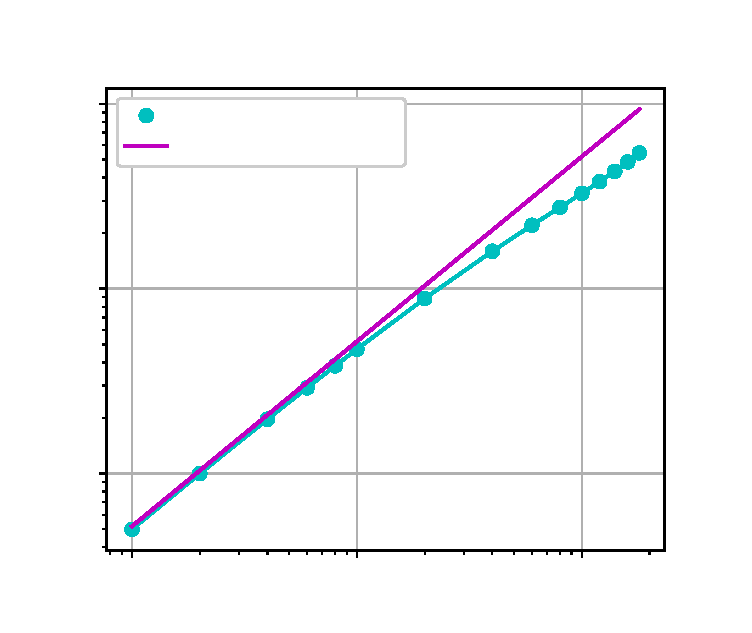
\includegraphics[width=\unitlength]{images_2ddl/lineaire.eps}}%
    \put(0.1257964,0.0485348){\color[rgb]{0,0,0}\makebox(0,0)[lb]{\smash{10}}}%
    \put(0.16297825,0.05963727){\color[rgb]{0,0,0}\makebox(0,0)[lb]{\smash{-2}}}%
    \put(0.43892111,0.04878857){\color[rgb]{0,0,0}\makebox(0,0)[lb]{\smash{10}}}%
    \put(0.47610296,0.05989104){\color[rgb]{0,0,0}\makebox(0,0)[lb]{\smash{-1}}}%
    \put(0.76074536,0.0485348){\color[rgb]{0,0,0}\makebox(0,0)[lb]{\smash{10}}}%
    \put(0.7979272,0.05963727){\color[rgb]{0,0,0}\makebox(0,0)[lb]{\smash{0}}}%
    \put(0.45736079,0.00605084){\color[rgb]{0,0,0}\makebox(0,0)[lb]{\smash{$\delta/R$ }}}%
    \put(0.05278422,0.18847651){\color[rgb]{0,0,0}\makebox(0,0)[lb]{\smash{10}}}%
    \put(0.08996607,0.19957897){\color[rgb]{0,0,0}\makebox(0,0)[lb]{\smash{2}}}%
    \put(0.05278422,0.44581787){\color[rgb]{0,0,0}\makebox(0,0)[lb]{\smash{10}}}%
    \put(0.08996607,0.45692033){\color[rgb]{0,0,0}\makebox(0,0)[lb]{\smash{3}}}%
    \put(0.05278422,0.70196636){\color[rgb]{0,0,0}\makebox(0,0)[lb]{\smash{10}}}%
    \put(0.08996607,0.71306882){\color[rgb]{0,0,0}\makebox(0,0)[lb]{\smash{4}}}%
    \put(0.03515632,0.373692){\color[rgb]{0,0,0}\rotatebox{90}{\makebox(0,0)[lb]{\smash{$F (N)$ }}}}%
    \put(0.23259861,0.68690835){\color[rgb]{0,0,0}\makebox(0,0)[lb]{\smash{étude éléments finis}}}%
    \put(0.23259861,0.64435615){\color[rgb]{0,0,0}\makebox(0,0)[lb]{\smash{théorie}}}%
  \end{picture}%
\endgroup%
